\documentclass[a4paper,11pt]{article}

\usepackage[a4paper,margin=2.3cm]{geometry}
\usepackage{graphicx}
\usepackage[section]{placeins}
\usepackage{cleveref}
\usepackage{listings}

\usepackage{graphicx}
\usepackage{hyperref}
\usepackage[capitalise, nameinlink, sort]{cleveref}
\usepackage{booktabs}
\usepackage{microtype}
\usepackage{subcaption}
\usepackage{tikz}
\usepackage{tabularx}
\usepackage{changepage}
\usepackage{xspace}
\usepackage{amssymb}
\newcommand{\ie}{\emph{i.e.}\@\xspace}
\newcommand{\eg}{\emph{e.g.}\@\xspace}
\makeatletter
\newcommand*{\etc}{\@ifnextchar{.}{etc}{etc.\@\xspace}}
\makeatother
\newcommand{\etal}{\emph{et al.}\@\xspace}

%%%%% fix for caption being too close to table
\usepackage{caption}
\captionsetup[table]{skip=5pt}
%%%% end fix

%\usepackage{pgfplotstable}
\usepackage{makecell}

\renewcommand\UrlFont{\color{blue}\rmfamily}

\title{Garbage Collection Results}
\author{Ruairidh MacGregor}
\date{}

\begin{document}

\maketitle

\section{Overview}

This document contains results for the NUMA garbage collection metrics, which are as follows:

\begin{description}
\item \textbf{GC Frequency (per region, per generation)}: this is illustrated in the form of a table. 
\item \textbf{GC Locality}: this is illustrated in the form of an access matrix $M$, where an entry $(i,j)$ in $M$ means a thread in region $i$ accessing objects in a remote region.
\end{description}

\section{Parfib}

\begin{table}[!htb]
  \centering
  \resizebox{\linewidth}{!}{
  \footnotesize
  \begin{tabular}{@{}c|cccccccc@{}}

  \makecel{Generation} & \makecell{Region 0} & \makecell{Region 1} & \makecell{Region 2} & \makecell{Region 3} & \makecell{Region 4} & \makecell{Region 5} & \makecell{Region 6} & \makecell{Region 7} \\
  \midrule
  1 & 4292 & 6850 & 7074 & 5197 & 4184 & 5119 & 7686 & 8695 \\
  2 & 56   & 78   & 55   & 59   & 48   & 41   & 77   & 68 \\
  \midrule
  \end{tabular}
  }
  \caption{Garbage Collection frequencies per region and per generation.}
  \label{table:baseline}
\end{table}

\begin{figure}[!htb]
    \centering
    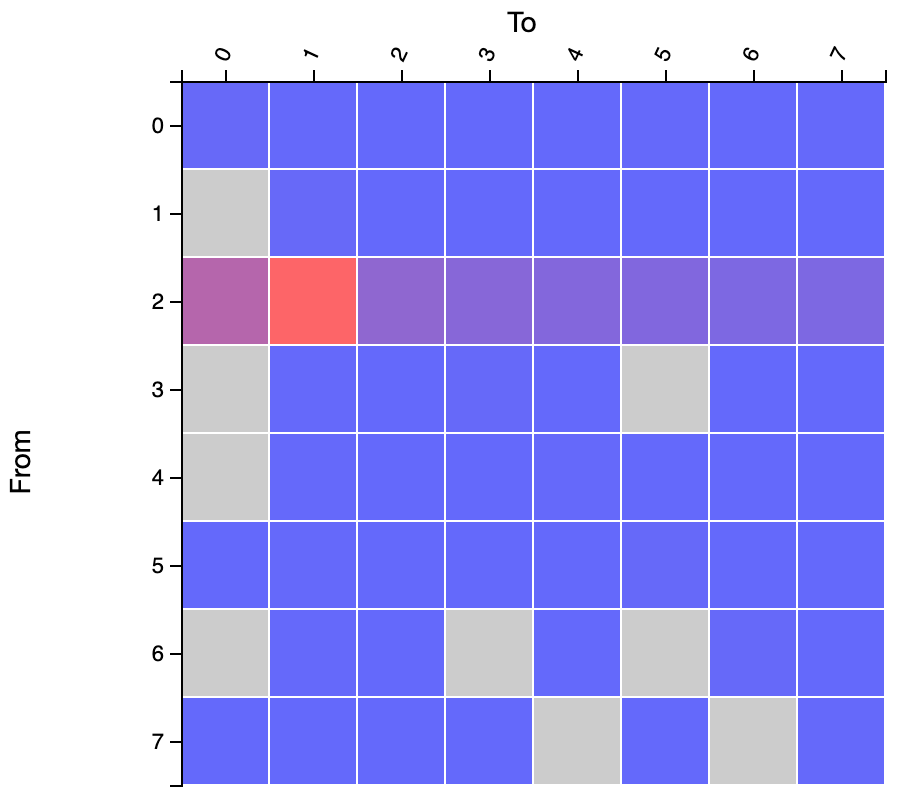
\includegraphics[width=0.6\linewidth]{TechMemo/gc/images/parfib_gc.png}
    \caption{Garbage Collection locality access matrix for Parfib benchmark.}
    \label{fig:my_label}
\end{figure}

\section{Blackscholes}

\begin{table}[!htb]
  \centering
  \resizebox{\linewidth}{!}{
  \footnotesize
  \begin{tabular}{@{}c|cccccccc@{}}

  \makecel{Generation} & \makecell{Region 0} & \makecell{Region 1} & \makecell{Region 2} & \makecell{Region 3} & \makecell{Region 4} & \makecell{Region 5} & \makecell{Region 6} & \makecell{Region 7} \\
  \midrule
  1 & 38 & 30 & 9 & 58 & 118 & 108 & 42 & 66 \\
  2 & 6  & 3  & 4 & 4  & 4   & 3   & 0 &  6 \\
  \midrule
  \end{tabular}
  }
  \caption{Garbage Collection frequencies per region and per generation.}
  \label{table:baseline}
\end{table}

\begin{figure}[!htb]
    \centering
    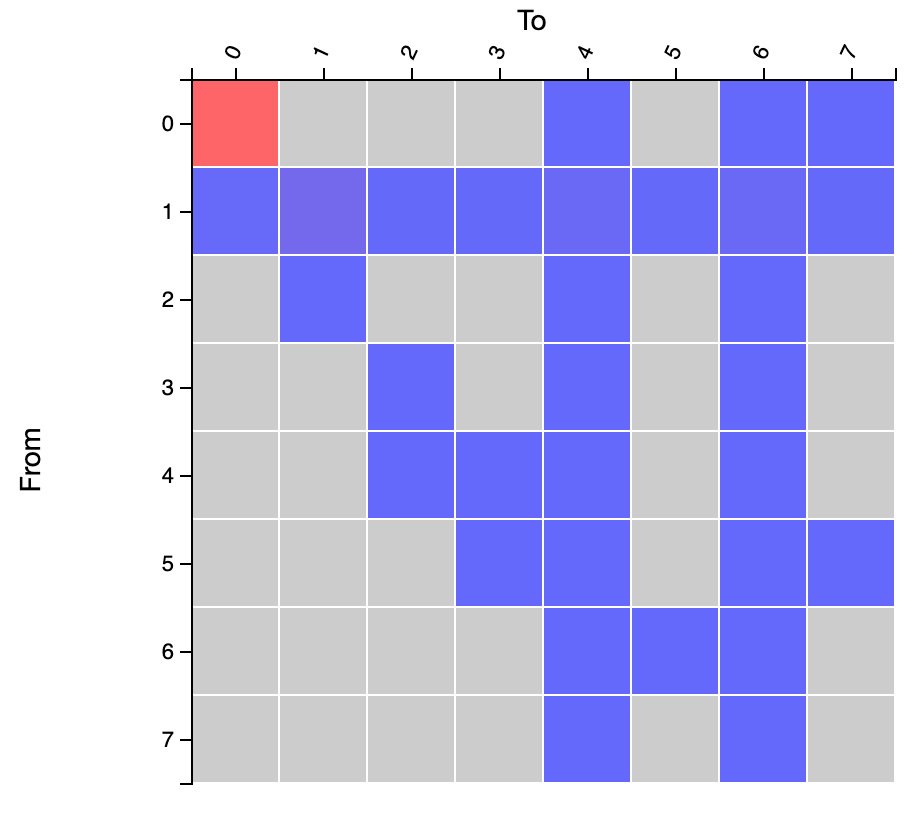
\includegraphics[width=0.6\linewidth]{TechMemo/gc/images/bscholes_gc.png}
    \caption{Garbage Collection locality access matrix for Blackscholes benchmark.}
    \label{fig:my_label}
\end{figure}

\section{Queens}

\begin{table}[!htb]
  \centering
  \resizebox{\linewidth}{!}{
  \footnotesize
  \begin{tabular}{@{}c|cccccccc@{}}

  \makecel{Generation} & \makecell{Region 0} & \makecell{Region 1} & \makecell{Region 2} & \makecell{Region 3} & \makecell{Region 4} & \makecell{Region 5} & \makecell{Region 6} & \makecell{Region 7} \\
  \midrule
  1 & 75 & 242 & 80 & 101 & 84 & 40 & 76 & 49 \\
  2 & 6  & 7   & 4  & 4   & 5  & 3  & 3  & 6 \\
  \midrule
  \end{tabular}
  }
  \caption{Garbage Collection frequencies per region and per generation.}
  \label{table:baseline}
\end{table}

\begin{figure}[!htb]
    \centering
    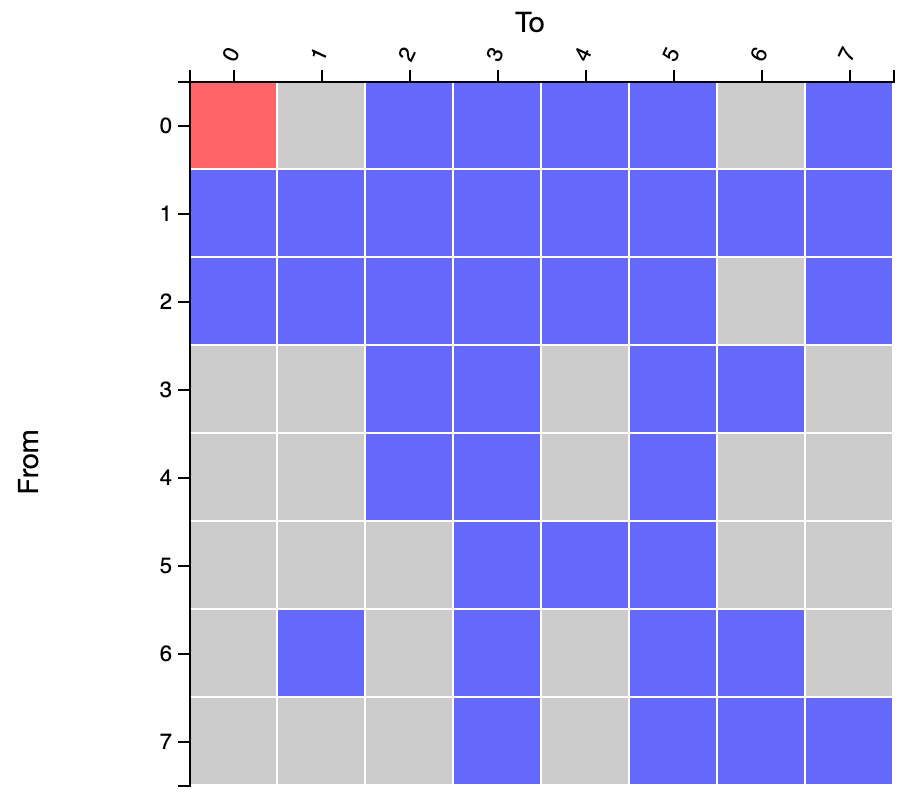
\includegraphics[width=0.6\linewidth]{TechMemo/gc/images/queens_gc.png}
    \caption{Garbage Collection locality access matrix for Queens benchmark.}
    \label{fig:my_label}
\end{figure}

\section{Partak}

\begin{table}[!htb]
  \centering
  \resizebox{\linewidth}{!}{
  \footnotesize
  \begin{tabular}{@{}c|cccccccc@{}}

  \makecel{Generation} & \makecell{Region 0} & \makecell{Region 1} & \makecell{Region 2} & \makecell{Region 3} & \makecell{Region 4} & \makecell{Region 5} & \makecell{Region 6} & \makecell{Region 7} \\
  \midrule
  1 & 5591 & 7277 & 5679 & 5782 & 5722 & 5898 & 5287 & 6084 \\
  2 & 104  & 124  & 115  & 122  & 115  & 132  & 117  & 89 \\
  \midrule
  \end{tabular}
  }
  \caption{Garbage Collection frequencies per region and per generation.}
  \label{table:baseline}
\end{table}

\begin{figure}[!htb]
    \centering
    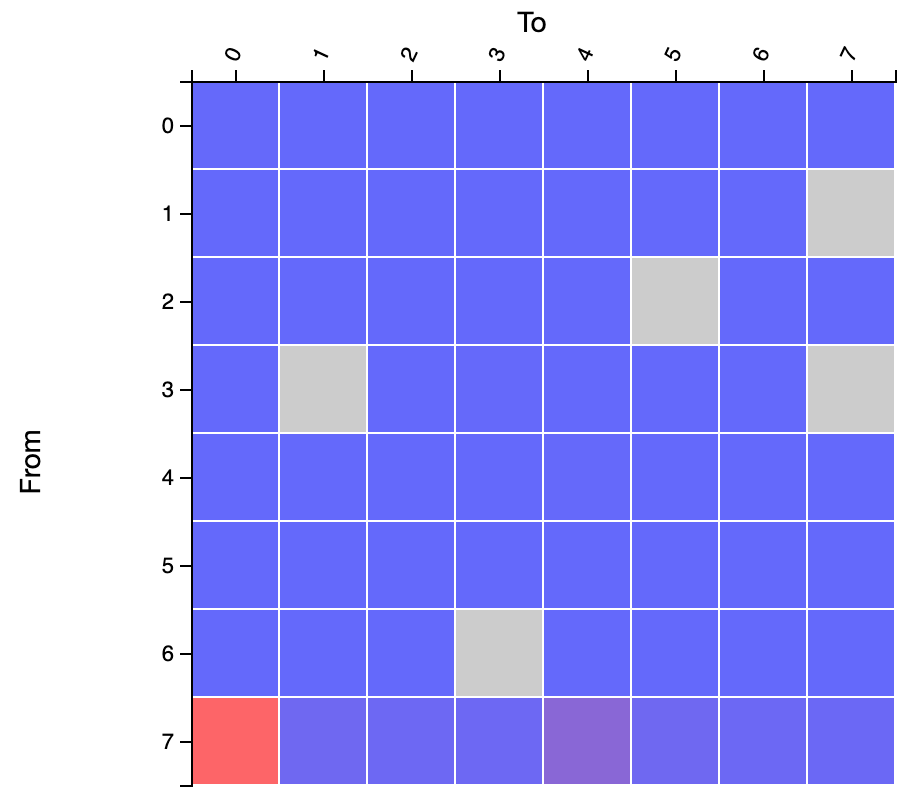
\includegraphics[width=0.6\linewidth]{TechMemo/gc/images/partak_gc.png}
    \caption{Garbage Collection locality access matrix for the Partak benchmark.}
    \label{fig:my_label}
\end{figure}

\section{Matmult}

\begin{table}[!htb]
  \centering
  \resizebox{\linewidth}{!}{
  \footnotesize
  \begin{tabular}{@{}c|cccccccc@{}}

  \makecel{Generation} & \makecell{Region 0} & \makecell{Region 1} & \makecell{Region 2} & \makecell{Region 3} & \makecell{Region 4} & \makecell{Region 5} & \makecell{Region 6} & \makecell{Region 7} \\
  \midrule
  1 & 771 & 2 & 4 & 1 & 0 & 1 & 3 & 3 \\
  2 & 10  & 2 & 4 & 1 & 0 & 1 & 3 & 3 \\
  \midrule
  \end{tabular}
  }
  \caption{Garbage Collection frequencies per region and per generation.}
  \label{table:baseline}
\end{table}

\begin{figure}[!htb]
    \centering
    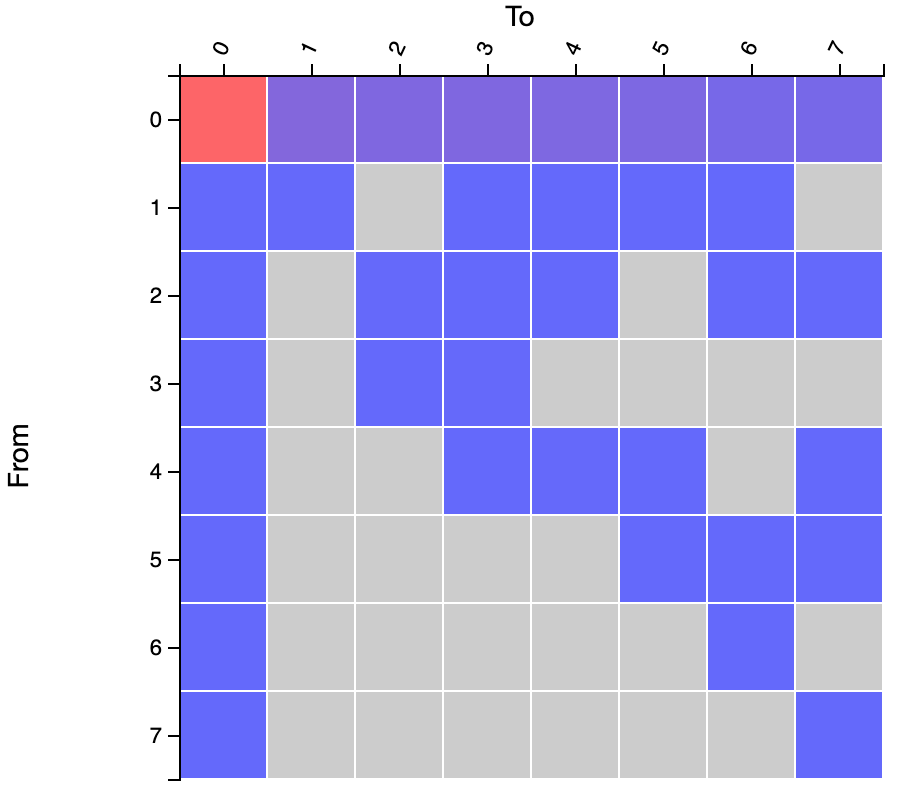
\includegraphics[width=0.6\linewidth]{TechMemo/gc/images/matmult_gc.png}
    \caption{Garbage Collection locality access matrix for the Matmult benchmark.}
    \label{fig:my_label}
\end{figure}

\section{Gray}

\begin{table}[!htb]
  \centering
  \resizebox{\linewidth}{!}{
  \footnotesize
  \begin{tabular}{@{}c|cccccccc@{}}

  \makecel{Generation} & \makecell{Region 0} & \makecell{Region 1} & \makecell{Region 2} & \makecell{Region 3} & \makecell{Region 4} & \makecell{Region 5} & \makecell{Region 6} & \makecell{Region 7} \\
  \midrule
  1 & 771 & 2 & 4 & 1 & 0 & 1 & 3 & 3 \\
  2 & 10  & 2 & 4 & 1 & 0 & 1 & 3 & 3 \\
  \midrule
  \end{tabular}
  }
  \caption{Garbage Collection frequencies per region and per generation.}
  \label{table:baseline}
\end{table}

\begin{figure}[!htb]
    \centering
    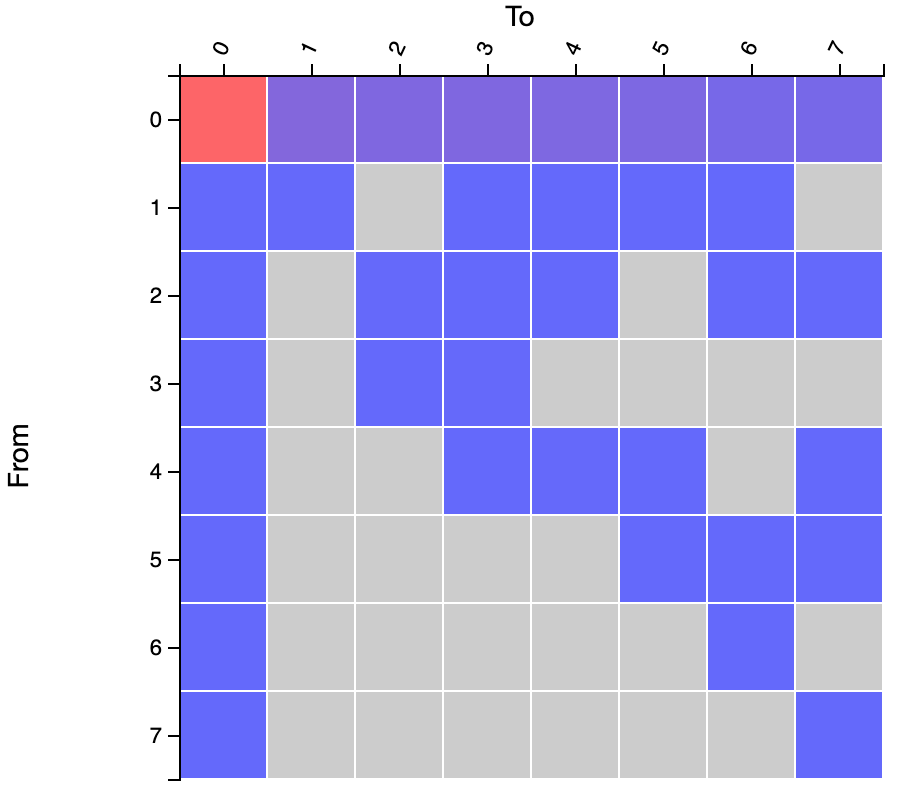
\includegraphics[width=0.6\linewidth]{TechMemo/gc/images/gray_gc.png}
    \caption{Garbage Collection locality access matrix for the Gray benchmark.}
    \label{fig:my_label}
\end{figure}

\section{Sumeuler}

\begin{table}[!htb]
  \centering
  \resizebox{\linewidth}{!}{
  \footnotesize
  \begin{tabular}{@{}c|cccccccc@{}}

  \makecel{Generation} & \makecell{Region 0} & \makecell{Region 1} & \makecell{Region 2} & \makecell{Region 3} & \makecell{Region 4} & \makecell{Region 5} & \makecell{Region 6} & \makecell{Region 7} \\
  \midrule
  1 & 2818 & 3481 & 3453 & 2684 & 3040 & 2969 & 3410 & 3887 \\
  2 & 11   & 2    & 4    & 6    & 5    & 6    & 7    & 6 \\
  \midrule
  \end{tabular}
  }
  \caption{Garbage Collection frequencies per region and per generation.}
  \label{table:baseline}
\end{table}

\begin{figure}[!htb]
    \centering
    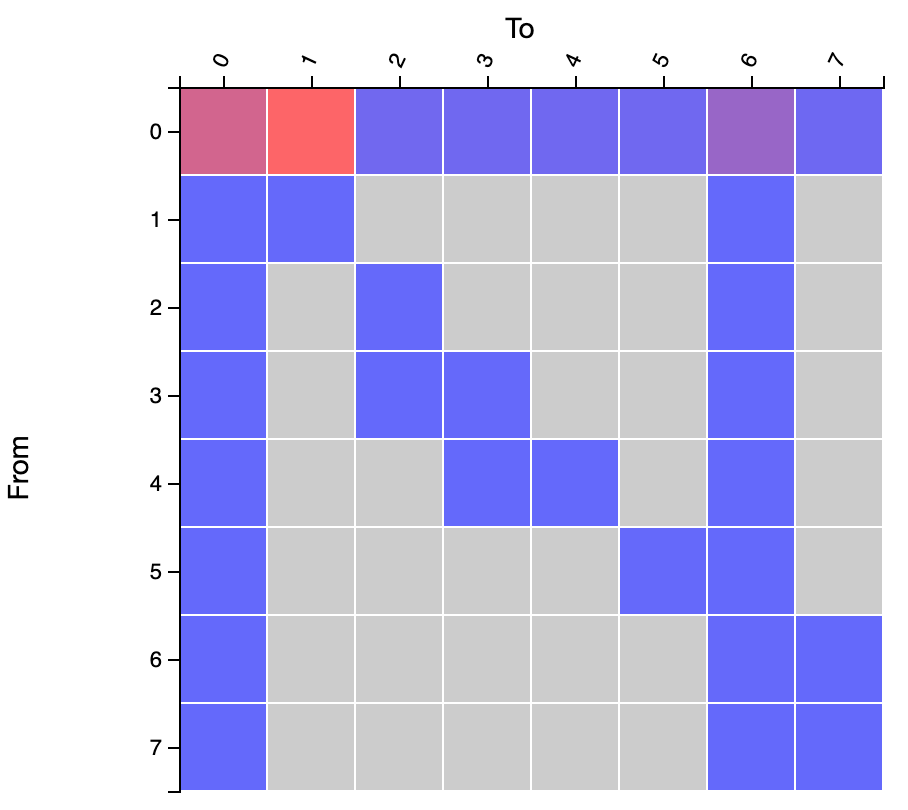
\includegraphics[width=0.6\linewidth]{TechMemo/gc/images/sumeuler_gc.png}
    \caption{Garbage Collection locality access matrix for the Gray benchmark.}
    \label{fig:my_label}
\end{figure}

\section{Mandel}

\begin{table}[!htb]
  \centering
  \resizebox{\linewidth}{!}{
  \footnotesize
  \begin{tabular}{@{}c|cccccccc@{}}

  \makecel{Generation} & \makecell{Region 0} & \makecell{Region 1} & \makecell{Region 2} & \makecell{Region 3} & \makecell{Region 4} & \makecell{Region 5} & \makecell{Region 6} & \makecell{Region 7} \\
  \midrule
  1 & 9 & 5  & 9  & 5  & 5  & 2  & 8  & 8  \\
  2 & 9 & 51 & 36 & 45 & 66 & 43 & 35 & 27 \\
  \midrule
  \end{tabular}
  }
  \caption{Garbage Collection frequencies per region and per generation.}
  \label{table:baseline}
\end{table}

\begin{figure}[!htb]
    \centering
    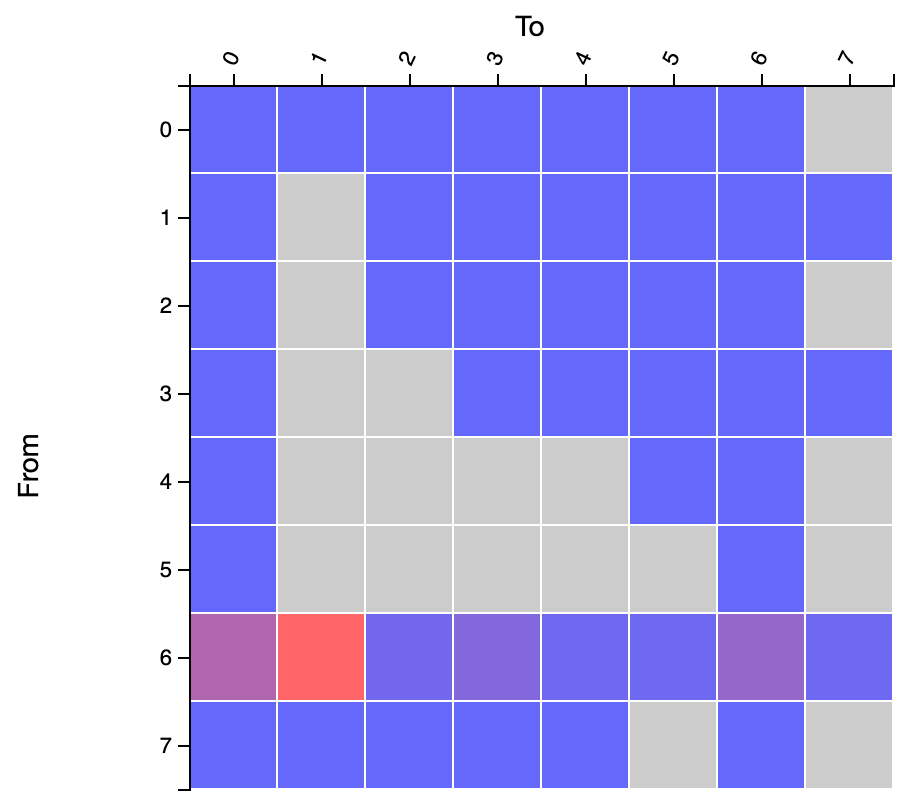
\includegraphics[width=0.6\linewidth]{TechMemo/gc/images/mandel_gc.png}
    \caption{Garbage Collection locality access matrix for the Gray benchmark.}
    \label{fig:my_label}
\end{figure}


\end{document}